\pagebreak
\noindent \underline{\textbf{Potensial Listrik}}
\vskip 10pt
\begin{enumerate}
    \item \underline{\textbf{Potensial \textit{Geiger Counter}}}
    \vskip5pt
    Suatu \textit{Geiger Counter} (alat pencacah partikel) terdiri dari logam berbentuk silinder dengan diameter $2.1cm$. Di sumbu silinder terdapat suatu kawat berdiameter $1.34\times10^{-4}cm$. Jika diantara logam dan kawat diberi tegangan $855V$, hitung besar medan listrik pada permukaan kawat dan permukaan silinder!
    \vskip8pt
    \begin{minipage}{0.3\textwidth}
    Muatan yang tersimpan
    \begin{align*}
        V&=-\int_{r_{k}}^{r_{s}}\vec{E}\cdot\vec{dr} \\
        &=-\int_{r_{k}}^{r_{s}}\frac{Q}{2\pi\varepsilon_{0}r}dr \\
        &=-\frac{Q}{2\pi\varepsilon_{0}}ln\left ( \frac{r_{k}}{r_{s}} \right )\\
        V&=\frac{Q}{2\pi\varepsilon_{0}}ln\left ( \frac{r_{s}}{r_{k}} \right )\\
        Q &= \frac{2\pi\varepsilon_{0}V}{ln\left ( \frac{r_{s}}{r_{k}} \right )}\\
        Q &= \frac{855\cdot2\cdot3.14\cdot8.85\times10^{-12}}{ln\left ( \frac{\frac{1}{2}\cdot2.1\times10^{-2}}{\frac{1}{2}\cdot1.34\times10^{-4}\times10^{-2}} \right )}\\
        Q &= 4.91\times10^{-9}C
    \end{align*}
    \end{minipage}
    \hfill
    \begin{minipage}{0.6\textwidth}
    a) Medan listrik pada permukaan silinder
        \begin{align*}
        E&=\frac{Q}{2\pi\varepsilon_{0}r}\\
        E&=\frac{4.91\times10^{-9}}{2\cdot\3.14\cdot8.85\times10^{-12}\cdot\frac{1}{2}\cdot1.34\times10^{-4}\times10^{-2}}\\
        E&=1.32\times10^{8}=132\times10^{6}V/m\\
        &\fbox{$E=132MV/m$}
        \end{align*}
    b) Medan listrik pada permukaan kawat
        \begin{align*}
        E&=\frac{Q}{2\pi\varepsilon_{0}r}\\
        E&=\frac{4.91\times10^{-9}}{2\cdot\3.14\cdot8.85\times10^{-12}\cdot\frac{1}{2}\cdot2.1\times10^{-2}}\\
        E&=8413.7V/m\\
        &\fbox{$E=8.41kV/m$}
        \end{align*}
    \end{minipage}


    \item \underline{\textbf{Muatan Menempel pada Pesawat Luar Angkasa}}
    \vskip5pt
    Suatu pesawat luar angkasa bergerak melewati sekumpulan gas yang terionisasi pada ionosfer bumi. Potensial pesawat ini berubah $-1$ \textit{Volt} saat ia menempuh satu putaran. Degan menganggap pesawat berbentuk bola berjari-jari $10m$, perkirakan berapa jumlah muatan yang dikumpulkannya!
    \vskip8pt
    \begin{minipage}{0.4\textwidth}
    \begin{align*}
        W &= \int\vec{F}\cdot\vec{dr}\\
        \Delta V &= \int\vec{E}\cdot\vec{dr}\\
        &=  \int\frac{kdq}{r}\\
        &= \int_{0}^{2\pi R}\frac{k\lambda}{R}dL\\
        &=\frac{k\lambda}{R}2\pi R\\
    \end{align*}
    \end{minipage}
    \hfill
    \begin{minipage}{0.6\textwidth}
    \begin{align*}
        \Delta V &= \frac{kQ}{R}\\
        -1&=\frac{9\times10^{-9}}{10}Q\\
        Q &= \frac{-10}{9\times10^{-9}}\\
        Q &= -1.11\times10^{-9}C\\
        &\fbox{$Q =-1.11nC$}
    \end{align*}
    \end{minipage}
    \pagebreak
    \item \underline{\textbf{Potensial tetesan air}}
    \vskip5pt
    Suatu tetes air membawa muatan $32.0pC$ mempunyai potensial $512V$ di permukaannya. Hitung jari-jari tetesan ini! Jika dua tetesan yang sejenis dengan jari-jari yang sama dengan tetesan di atas bergabung menjadi satu tetes besar. Hitung potensial pada tetes yang baru!
    \begin{align*}
        V&=\frac{kQ}{R}\\
        R&=\frac{kQ}{V}\\
        &= \frac{9\times10^{9}\cdot32\times10^{-12}}{512}\\
        &=0.000562m\\
        &\fbox{$R=0.562mm$}
    \end{align*}

    Tetesan air bergabung menjadi satu muatan yang lebih bisa. Dengan menganggap rapat muatan mula-mula dan ketika sudah bergabung adalah sama maka
    \begin{minipage}{0.5\textwidth}
    \begin{align*}
        \rho_{awal}=\rho_{baru}\\
        \frac{Q_{awal}}{V_{awal}}=\frac{Q_{baru}}{V_{baru}}\\
        \frac{Q}{\frac{4}{3}\pi R^{3}}=\frac{2Q}{\frac{4}{3}\pi r^{3}}\\
        \frac{Q}{R^{3}}=\frac{2Q}{r^{3}}\\
        r^{3}=2R^{3}\\
        r=2^{\frac{1}{3}}R\\
    \end{align*}
    \end{minipage}
    \hfill
    \begin{minipage}{0.3\textwidth}
    \begin{align*}
        V &= \frac{k(2Q)}{r}\\
        V &= \frac{2\cdot512}{2^{\frac{1}{3}}}\\
        &\fbox{$V= 813V$}
    \end{align*}
    \end{minipage}

    \item \underline{\textbf{Potensial Gelembung Sabun}}
    \vskip5pt
    Suatu gelembung sabun berjari-jari $10cm$ dengan ketebalan $3.3\times 10^{-6}cm$ diberi muatan sampai mencapai potensial sebesar $100V$. Gelembung ini kemudian pecah dan menjadi suatu tetesan berbentuk bola. Hitung potensial tetesan ini!.

    \begin{center}
    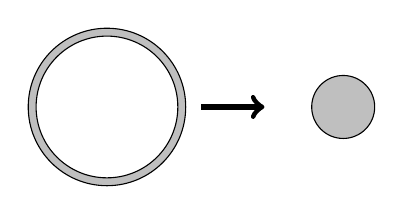
\begin{tikzpicture}
    \filldraw[fill=gray!50] (0,0) circle [radius=1cm];
    \filldraw[fill=white] (0,0) circle [radius=0.9cm];
    \filldraw[fill=gray!50] (3,0) circle [radius=0.4cm];
    \draw [line width=2pt,->](1.2,0)--(2,0);
    \end{tikzpicture}
    \end{center}

    Gelembung (kulit bola) dipecahkan sehingga menjadi tetesan berbentuk bola. Maka muatan gelembung = muatan tetesan dan volume gelembung = volume tetesan.

    \begin{minipage}{0.4\textwidth}
    Volume gelembung (kulit bola) dan Volume tetesan (bola) sama
    \begin{align*}
        v_{gelembung}&=v_{tetesan}\\
        4\pi R^{2}\cdot t &= \frac{4}{3}\pi r^{3}\\
        r^{3}&=3R^{2}t\\
        r&=(3R^{2}t)^{1/3}
    \end{align*}

    \end{minipage}
    \hfill
    \begin{minipage}{0.4\textwidth}
    Potensial gelembung dan tetesan
    \begin{align*}
        V_{gelembung}&=\frac{kQ}{R}\\
        V_{tetesan}&=\frac{kQ}{r}\\
    \end{align*}
    \end{minipage}
    \vskip15pt
    Sehingga potensial dari tetesan
    \begin{align*}
        V_{gelembung}R &= V_{tetesan}r\\
        V_{tetesan}&=\frac{R}{r}V_{gelembung}\\
        &=\frac{R}{(3R^{2}t)^{1/3}}V_{gelembung}\\
        &=\frac{10\times10^{-2}}{(3\cdot (10\times10^{-2})^{2}(3.3\times10^{-6}\times10^{-2}))^{1/3}}100\\
        &=10033.55\\
        &\fbox{V\approx 10kV}
    \end{align*}
\end{enumerate}